% % % % % % % % % % % % % % % % % % % % % % % % % % % % % % % % % % % % % % % %
\section{A gentle introduction}

Let us start with an example that is, in some of its many forms, a must
in any text about linear programming. Let us have a student  
going to pull an all-nighter in preparation for some exam. In order to 
stay awake he needs to get at least 
$270$~mg of caffeine, and at least $120$~g of sugar. At the same time,
a dose of more than $180$~mg of aspartame may be hazardous to his health. 
He can choose between two drinks: brown stuff for \hbox{\EUR{$1$}/dl}, and
green stuff for \hbox{\EUR{$1,50$}/dl.}
1 dl of brown stuff contains  $30$~mg of caffeine, $40$~g of sugar, and
$40$~mg of aspartame, while the same amount of green stuff contains
$90$~mg of caffeine, $30$~g of sugar, and $30$~mg of aspartame. 
How much of which stuff should the student buy in order to satisfy all his needs
at the smallest possible cost?
If he buys $x$~dl of brown stuff, and $y$~dl of green stuff, the problem
(called a {\em linear program}) can be formulated as follows:


\begin{equation}
  \label{eq:LP:1}
\begin{array}{rccccll}
                          & \multicolumn{3}{c}{\text{dl of stuff}} \\ 
                          & \text{brown} & & \text{green}\\
  {\rm minimize}     & x   & + & 1.5 y & =: & f(x,y) &  \text{\em price}\\
  {\rm subject\ to} & \color{blue}{30 x } & \color{blue}{+} & \color{blue}{90 y} & \color{blue}{\ge} & \color{blue}{270} & \text{\color{blue}{\em caffeine}}\\ 
                           & \color{red}{40 x}   & \color{red}{+}  & \color{red}{30 y}  & \color{red}{\ge} & \color{red}{120} & \text{\color{red}{\em sugar}} \\
                           & \color{magenta}{40 x} & \color{magenta}{+} & \color{magenta}{30 y} & \color{magenta}{\le} & \color{magenta}{180} & \text{\color{magenta}{\em aspartame}}\\
                          &      &   & x,y  &\ge& 0
\end{array}
\end{equation}
%
It is easy to see that, e.g., $4$~dl of green stuff satisfy all the requirements
at the cost of \EUR{6}, while providing even more caffeine than necessary, and
less aspartame than allowed. On the other hand, if the student would be buying
only brown stuff, in order to satisfy his needs for caffeine he would have
to buy 9~dl of it, which would overdose him with aspartame (and it would be
too costly anyway).
When looking for the optimal optimal solution the following geometric interpretation
comes handy: to each solution with $x$~dl of brown stuff, and $y$~dl of green stuff
assign a point $(x,y)$ in the plane. Each of the constraints then defines a half-plane
where a feasible solution can be located. Hence, all feasible solutions lie in the
quadrilateral on the left:


% draws a halfplane
% optional: paameters to draw
% fist point, second point, orientation (+/-), length1, length2
\newcommand{\halfplane}[6][ ]{%
  \coordinate (O) at (#2);
  \coordinate (XX) at (#3);
  \coordinate (YY) at ($ (O) !1! 90:(XX) $);
  \coordinate (X) at ($ (XX) - (O) $);
  \coordinate (Y) at ($ (YY) - (O) $);
  \coordinate (E) at ($ (XX)!#6! ($(XX)+(X)$) $);
  \begin{scope}[#1]
      \draw 
          ($ (O)!-#5!(XX) $) -- (E);
     
      \foreach \i in {0,0.1,...,1}  
          \draw
          let
              \p1 = ($ ($ (E) !1.5cm! (O) $) + ($ (0,0) !\i cm! (X) $) $)
         in
              (\p1) -- ($ (\p1) ! 8pt ! #4 330:($ (\p1)+($ (0,0)#4(Y) $) $) $);
  \end{scope}
}


\renewcommand{\common}{%
  %axis
  \draw (-2,0) -- coordinate (x axis mid) (11,0);
  \draw (0,-2) -- coordinate (y axis mid) (0,8);
  %ticks
  \foreach \x in {-2,...,10}
      \draw (\x,1pt) -- (\x,-3pt);
  \foreach \x in {2,4,...,10}
      \draw (\x,-3pt) node[anchor=north] {\x};
  \foreach \y in {1,...,7}
      \draw (1pt,\y) -- (-3pt,\y) 
          node[anchor=east] {\y}; 
      \draw (0,0) node[anchor=north east]{$0$};
  %labels      
      \node[below=0.8cm] at (x axis mid) {brown stuff};
  \node[rotate=90] at (-2,4) {green stuff};
  
  \filldraw[fill=black!50, line width=0.8pt, fill opacity=0.5 ]
    (0,6) -- (0,4) -- (1,2.66) -- (3,2) -- cycle;
}


\begin{center}
\begin{tikzpicture}[scale=0.5]

  \halfplane[color=red]{0,4}{3,0}{+}{1cm}{1cm}
  \halfplane[color=blue]{9,0}{0,3}{-}{1cm}{1cm}
  \halfplane[color=magenta]{0,6}{4.5,0}{-}{1cm}{1cm}

  \common
\end{tikzpicture}
\hfill
\begin{tikzpicture}[scale=0.5]
  \begin{scope}
    \clip (-1,-0.4) -- (11,-0.4) -- (11,8) -- (-1,8) -- cycle;
    \coordinate (v) at (3,-2);
    \draw[dashed,color=black!80]  
        \foreach \p in {(1,2.66),(0,4),(0,6),(0,7)}
            {($ (\p ! 20cm ! ($ (\p - (v) $) $)  -- ($ (\p ! 20cm ! ($ (\p + (v) $) $)};
    \coordinate (q) at ($ (0,7) !4cm! ($ (0,7) + (v) $) $);
    \draw[thick,->]
        (5,6) node[anchor=south west] {$f(x,y)=10.5$}  -- (q) ;
  \end{scope}
  
      
  \common
  \filldraw[very thin,red,dotted]
        (1,2.66) circle (2pt) -- (0,2.66)
        (1, 2.66) -- (1,0);
\end{tikzpicture}
\end{center}
%
At the same time we know that $f(x,y)=x+1.5y$ is a linear function, so points
with the same value of $f$ form a straight line (see the right figure). Now it should
be clear that in order to find the optimal solution it is sufficient to
to check the four corners of the quadrilateral and conclude that the best thing
to do is to buy $1$~dl of brown stuff, and $2\frac{2}{3}$~dl of green stuff for \EUR{5}.


\noindent
\begin{minipage}[t]{\textwidth-6cm}
\vspace{0pt}
The previous ideas lead directly to a simple algorithm for solving the problem with
two variables, and a number of inequality constraints: for each constraint consider the
corresponding half-plane, construct the (convex) polygon that is the intersection 
of all these halfplanes, and choose the optimal solution from among all its vertices.
With three variables, the constraints are of the form $a_1x+a_2y+a_3z\ge b$, and they 
define half-spaces in 3D, whose intersection is a polyhedron. Points with the
same value of the function $f(x,y,z)=c_1x+c_2y+c_3z$ form a plane, and so it is sufficient to
check all the vertices of the polyhedron to find the optimal solution.\\
\end{minipage}
\begin{minipage}[t]{6cm}
  \vspace{0pt}
  % origin, side (vector), second side
\newcommand{\kvad}[3]{%
    (#1) -- ($ (#1) + (#2) $) -- ($ (#1) + (#2) + (#3) $) -- ($ (#1) + (#3) $) -- cycle
}

% new_point_name x y z  (RotatedOriginShift should be set)
\newcommand{\rottomain}[4]{
    \tdplottransformrotmain{#2}{#3}{#4}
    \coordinate (#1) at ($ (\tdplotresx,\tdplotresy,\tdplotresz) + (RotatedOriginShift) $);
}

% intersection of two lines: name and four endpoints
\newcommand{\intersect}[5]{
    \path [name path=intersect_p1] (#2) -- (#3);
    \path [name path=intersect_p2] (#4) -- (#5);
    \path [name intersections={of=intersect_p1 and intersect_p2, by={#1}} ];
}

\renewcommand{\axes}{%
    \draw[thick,->] 
      (0,0,0) -- (1.3,0,0) node[anchor=north east]{$x$}
      (0,0,0) -- (0,1.3,0) node[anchor=north west]{$y$}
      (0,0,0) -- (0,0,1.3) node[anchor=south]{$z$};
    \draw[thick,->,tdplot_rotated_coords,color=blue] 
      (0,0,0) -- (1,0,0) node[anchor=north east]{$x$}
      (0,0,0) -- (0,1,0) node[anchor=north west]{$y$}
      (0,0,0) -- (0,0,1) node[anchor=south]{$z$};
}

\begin{center}
  \tdplotsetmaincoords{70}{60}
  \begin{tikzpicture}[scale=2,tdplot_main_coords]

    \tdplotsetrotatedcoords{45}{55}{5}    
    \coordinate (RotatedOriginShift) at (1,1,1);
    \tdplotsetrotatedcoordsorigin{(RotatedOriginShift)}
    %\axes       

    \fill[fill=black!30,fill opacity=0.3]
        \kvad{0,0,0}{1,0,0}{0,1,0}
        \kvad{0,0,0}{0,1,0}{0,0,1}
        \kvad{1,1,1}{-1,0,0}{0,0,-1}
        \kvad{1,1,1}{0,-1,0}{0,0,-1};
    \fill[fill=black!90, fill opacity=0.3]
        \kvad{0,0,0}{1,0,0}{0,0,1};
    \fill[fill=black!50, fill opacity=0.3]
        \kvad{0,0,1}{1,0,0}{0,1,0};
        

  
    % blue kvad  
    \rottomain{p1}{-0.7}{-1}{0} % origin
    \rottomain{p2}{0.7}{-1}{0}  % o + x
    \rottomain{p3}{-0.7}{1}{0}  % o + y

    \intersect{i1}{p1}{p2}{1,0,1}{1,1,1}
    \intersect{i2}{p1}{p3}{0,0,1}{0,1,1}
    \intersect{i3}{p1}{p2}{1,1,0}{1,1,1}

    \draw
        (1,0,1) -- (i1)
        (0,0,1) -- (i2)
        (1,1,0) -- (i3)
        \kvad{0,0,0}{1,0,0}{0,0,1}
        (1,0,0) -- (1,1,0);

    \draw[dashed]    
        (i1) -- (1,1,1)
        (0,1,0) -- (1,1,0)
        (0,1,0) -- (0,0,0)
        (0,1,0) -- (0,1,1)
        (i2) -- (0,1,1)
        (i3) -- (1,1,1)
        (0,1,1) -- (1,1,1);

    \begin{scope}[tdplot_rotated_coords]
       \filldraw[color=blue,very thin,fill=blue!20,fill opacity=0.5]
          \kvad{-0.7,-1,0}{1.4,0,0}{0,2,0};
        %\draw[color=blue,very thick,->]  
        %  (0,0,0) -- (0,0,1);
        \fill[color=blue]
          (0,0,0) circle (1pt);
    \end{scope}


  \end{tikzpicture}
\end{center}

\end{minipage}


\noindent 
With increasing the number of variables, however, many problems arise, and it
soon becomes clear that a straightforward generalization is a road to hell. 
Let us have a different look at the geometry of the linear program. First, 
let us rewrite program (\ref{eq:LP:1}) to an equivalent form as follows:
multiply the function $f(x,y)$ by -1, and from minimization problem we get a maximization.
Then also premultiply by -1 the first and second constraint to get all the constraints
(except those $x,y\ge0$) in the ``$\le$'' form. Finally, since in each constraint the 
left hand side is smaller than the right hand side, we can add a new non-negative variable 
to represent the difference between the right hand side and the left hand side. These
transformations yield the following linear program which is obviously equivalent to the original one:

\begin{equation}
\label{eq:LP:2}
\begin{array}{rrrrrrcl}
  {\rm maximmize}     & -x   & -  1.5y &         &         &       & =: & f(x,y,s_1,s_2,s_3) \\
   {\rm subject\ to}& -30x & -  90y  & +   s_1 &         &       & =  & -270\\
                          & -40x & -  30y  &         & +   s_2 &       & =  & -120\\
                          &  40x & +  30y  &         &         &+  s_3 & =  & 180\\      
                          &      &         &     \multicolumn{3}{r}{x,y,s_1,s_2,s_3}  &\ge& 0
\end{array}
\end{equation}
%
If we denote
\begin{align*}
 \bm{c}&=\cvect{-1\\-1.5\\0\\0\\0}
&A&=\left(\begin{array}{ccccc}-30&-90&1&0&0\\-40&-30&0&1&0\\30&40&0&0&1\end{array}\right)
&\bm{b}&=\cvect{-270\\-120\\200}
\end{align*}
then the program (\ref{eq:LP:2}) can be written concisely
$$\max_{\bm{x}\in\R^5}\left\{ \bm{c}\tr\bm{x} \mid A\bm{x}=\bm{b},\; \bm{x}\ge0
\right\}.$$ 
The transformation increased the dimension of the problem from 2 to 5 (and we lost the possibility
of a graphical solution), but the gain is a nicer set of feasible solutions: feasible solutions
are non-negative solutions of a system of linear equations. In our case the matrix $A$ has rank 3
(the rows are linearly independent) and the solutions of the system
$A\bm{x}=\bm{b}$ 
form a two-dimensional subspace
$\bm{o}+c_1\bm{\alpha}+c_2\bm{\beta}$ where
\begin{align*}
\bm{o}&=\cvect{0\\0\\-270\\-120\\180}
      &\bm{\alpha}&=\cvect{1\\0\\30\\40\\-40}
      &\bm{\beta}&=\cvect{0\\1\\90\\30\\-30}.
\end{align*}
In other words, the feasible solutions of program (\ref{eq:LP:1}) 
form a 2-dimensional polygon (quadrilateral) in a 2-dimensional subspace (a plane),
while the feasible solutions of program (\ref{eq:LP:2}) form a 2-dimensional 
polygon \dom in a 5-dimensional space, where \dom is the intersection of a (2-dimensional)
plane with the positive orthant\footnote{in the same spirit as ''quadrant'' in 2D, and ''octant''
in 3D, we use the term ''orthant'' in a general $n$-dimensional space}. 
To illustrate this, consider the following simple programs (we show only the constraints, the 
utility function does not matter in this case):


\renewcommand{\commonii}{%
  %axis
  \draw (-0.5,0) -- coordinate (x axis mid) (1.5,0);
  \draw (0,-0.2) -- coordinate (y axis mid) (0,1.5);
  %ticks
  \foreach \x in {-0.2,-0.1,...,1.4}
      \draw (\x,1pt) -- (\x,-3pt);
  \draw (1,-3pt) node[anchor=north] {1};

  \foreach \y in {0.2,0.3,...,1.4}
      \draw (1pt,\y) -- (-3pt,\y);
  \draw (-1pt,1) node[anchor=east] {1}; 
  
  \draw (0,-3pt) node[anchor=north east]{$0$};
}


\renewcommand{\axes}{
    \draw
      (0,0,0) -- (1.5,0,0) node[anchor=north east]{$x$}
      (0,0,0) -- (0,1.5,0) node[anchor=north west]{$y$}
      (0,0,0) -- (0,0,1.5) node[anchor=south]{$s$};
}


\setlength{\picx}{(0.5\textwidth - 3cm)/2}
\setlength{\picy}{\picx}
\begin{tikzpicture}[x=\picx,y=\picy]
  \fill[fill=blue!50, opacity=0.8]
    (0,0) -- (1,0) -- (0,1) -- cycle;
  \commonii
  \draw[thick, shorten >= -10pt, shorten <= -10pt] (0,1) -- (1,0);
  \draw (0.7,1) node {$\begin{array}{rl}x+y&\le 1\\ x,y&\ge0\end{array}$};
  \foreach \p in {(0,0),(1,0),(0,1)}
    \filldraw \p circle (1.5pt); 
\end{tikzpicture}
\hfill
\tdplotsetmaincoords{70}{120}
\begin{tikzpicture}[scale=2.3,tdplot_main_coords]
  \axes
  \coordinate (u) at ($ (0,0,0)!2.5cm!(-1,1,0) $);
  \coordinate (v) at ($ (0,0,0)!2cm!(-1,-1,2) $);
  \coordinate (p) at ($ (1,0,0)!7mm! ($ (1,0,0)-($(u)+(v)$) $) $);
  
  \filldraw[fill=blue!30, opacity=0.3]
      (p) -- ($ (p) + (u) $) -- ($ (p) + (u) + (v) $) -- ($ (p) + (v) $) -- cycle;
  \draw[thin]
      (p) -- ($ (p) + (u) $) -- ($ (p) + (u) + (v) $) -- ($ (p) + (v) $) -- cycle;

  \filldraw[thick,fill=blue!50, opacity=0.8]
      (1,0,0) -- (0,1,0) -- (0,0,1) -- cycle;
  \foreach \p in {(1,0,0),(0,1,0),(0,0,1)}
    \filldraw \p circle (.8pt); 
 
   \draw[tdplot_screen_coords] (0.7,1) node {$\begin{array}{rl}x+y+s&= 1\\ x,y,s&\ge0\end{array}$};

\end{tikzpicture}

\noindent 
On the left there is a program with two variables and a 2-dimensional solution space. 
After the transformation into three dimensions the solution space remained 2-dimensional,
and it is the intersection of a plane with the positive octant. In the next example
the original problem has a 1-dimensional solution space. After the transformation into three
dimensions it is still 1-dimensional, and it is an intersection of a line with the positive octant.

\begin{tikzpicture}[x=\picx,y=\picy]
  \fill[fill=blue!30, opacity=0.3]
    (0,0) -- (1,0) -- (0,1) -- cycle;
  \draw[shorten >= -2cm, shorten <= -3pt] (0,0) -- (.5,.5);
  \draw[very thick]
    (0,0) -- (0.5,0.5);
  \commonii
  \draw[shorten >= -10pt, shorten <= -10pt] (0,1) -- (1,0);

  \draw (0.6,1.5) node {$\begin{array}{rl}x+y&\le 1\\ x-y&=0\\x,y&\ge0\end{array}$};
  \foreach \p in {(0,0),(.5,.5)}
    \filldraw \p circle (1.5pt); 
\end{tikzpicture}
\hfill
\tdplotsetmaincoords{70}{120}
\begin{tikzpicture}[scale=2.3,tdplot_main_coords]
  \axes
  \coordinate (u) at ($ (0,0,0)!2.5cm!(-1,1,0) $);
  \coordinate (v) at ($ (0,0,0)!2cm!(-1,-1,2) $);
  \coordinate (p) at ($ (1,0,0)!7mm! ($ (1,0,0)-($(u)+(v)$) $) $);
  
  \filldraw[fill=blue!30, opacity=0.3]
      (p) -- ($ (p) + (u) $) -- ($ (p) + (u) + (v) $) -- ($ (p) + (v) $) -- cycle;
  \draw[thin]
      (p) -- ($ (p) + (u) $) -- ($ (p) + (u) + (v) $) -- ($ (p) + (v) $) -- cycle;

  \coordinate (u) at ($ (0,0,0)!1cm!(1,1,0) $);
  \coordinate (v) at ($ (0,0,0)!1.8cm!(0,0,1) $);
  \coordinate (p) at ($ (0,0,0)!3mm! ($ (0,0,0)-($(u)+(v)$) $) $);
  
  \filldraw[fill=green!30, opacity=0.3]
      (p) -- ($ (p) + (u) $) -- ($ (p) + (u) + (v) $) -- ($ (p) + (v) $) -- cycle;
  \draw[thin]
      (p) -- ($ (p) + (u) $) -- ($ (p) + (u) + (v) $) -- ($ (p) + (v) $) -- cycle;
  

  \filldraw[color=blue!60, fill=blue!50, opacity=0.5]
      (1,0,0) -- (0,1,0) -- (0,0,1) -- cycle;
  \filldraw[color=green!60, fill=green!50, opacity=0.5]
      (0,0,0) -- (0,0,1) -- (.5,.5,0) -- cycle;


  \foreach \p in {(0,0,1),(.5,.5,0)}
    \filldraw \p circle (.8pt); 
 
  \draw[tdplot_screen_coords] (0.7,1.05) node {$\begin{array}{rl}x+y+s&=1\\ x-y&=0\\x,y,s&\ge0\end{array}$};
  \draw[very thin, dashed] 
      (0,0,0) -- (1.5,1.5,0)
      (0,0,0) -- (0,0,1)
      (1,0,0) -- (0,1,0) -- (0,0,1) -- cycle;
  \draw[very thick]
    (0,0,1) -- (0.5,0.5,0);

\end{tikzpicture}

\noindent 
The advantage of this form of the linear program is that it is easier to 
identify the vertices of the polygon of feasible solutions: they lie in some face of 
the form $x_i=0$.

Before continuing in our musings it is good to note that we may, without loss of generality,
suppose that the rows of the matrix $A$ are linearly independent:
if there is a row that is a linear combination of some other rows, then either there is
no feasible solution at all, or by leaving out that row the set of feasible solutions 
remains the same. We can summarize our ideas, and define a {\em normal form} of a linear program
as follows:

\vskip 1em
\noindent
\begin{framed}
  \begin{dfn}
  \label{df:LP:eqnormalform}
  A linear program is in the {\bf normal form}, if it is written as
\begin{equation}
  \max_{\bm{x}\in\R^n}\left\{ \bm{c}\tr\bm{x} \mid A\bm{x}=\bm{b},\;\bm{x}\ge\bm{0}\right\},
\end{equation}
where $A\in\R^{m\times n}$ has rank $m$. The set of feasible solutions $\dom=\left\{\bm{x}\in\R^n \mid  A\bm{x}=\bm{b},\;\bm{x}\ge\bm{0}\right\}$.
\end{dfn}
\end{framed}

\begin{itemize}
\item {\bf The goal is maximization.} 
  If the original goal was to minimize a linear function
$f(\bm{x})$, 
the new goal is to maximize the (linear) function
$-f(\bm{x})$.
\item {\bf All variables are non-negative.} 
Each variable $x$ that is not bound by a constraint $x\ge0$
will be replaced by two variables $p_x, q_x\ge0$, and each occurrence
of $x$ in will be replaced by $p_x0q_x$.
\item {\bf Each constraint, except for those $x\ge0$ has the form of equality}.
  A constraint of the form $\sum_ia_ix_i\ge b$ is first multiplied by $-1$ on
  both sides, turning it into $\sum_i-a_ix_i\le-b$. After all constraints
  have the inequalities facing the same direction, a new variable $s$ ({\em slack})
  is introduced for each constraint $\sum_ia_ix_i\le b$; this variable represents
  the extent to which the equality is violated, \ie 
 $s\ge 0$, and $s+\sum_ia_ix_i=b$.  
\item {\bf The matrix \bm{A} has full rank, \ie has \bm{m} linearly independent rows.}
\end{itemize} 

\noindent 
Now let us have a program in the normal form. In a way similar to the opening example,
we want to find the set of vertices (corners) of the polyhedron \dom of the feasible solutions,
so it is sufficient to check those vertices in order to find the optimal solution.
Since \dom is formed by the intersection of the solution space of the system $A\bm{x}=\bm{b}$
with the positive orthant, its corners have some (at least one)  coordinates 
$x_{i_1},\ldots,x_{i_k}$ zero (the hyperplane $x_i=0$ is on the border of the orthant). 
Moreover, the corners are ''pointy'' (unlike the points in some face $x_i=0$ where, say,
a whole line segment lies). The ''pointyness'' of a vertex can be formulated the following
way: if the constraints $A\bm{x}=\bm{b}$
are augmented by the set of equations  $x_{i_1}=0,\ldots,x_{i_k}=0$,
the resulting system has a unique solution (\ie a ''corner'' lies in the 
intersection of some of the boundary faces of the orthant, and no other point lies
in the same intersection). Since $A$ has full rank $m$, in order to have a unique
solution of the system, we need $k=n-m$. 

\noindent Now let us get back to program (\ref{eq:LP:2}).  The matrix $A$ has rank 3,
so the vertices of \dom are obtained by augmenting the system  $A\bm{x}=\bm{b}$ 
by two constraints $x_i=0$, and $x_j=0$. In this way, 10 different equation systems can 
be obtained, with the following solutions:


\vskip 1ex
{
\renewcommand{\arraystretch}{1.5}
\renewcommand{\tmp}[3]{\multicolumn{1}{#1>{\columncolor[gray]{0.9} $}#2<{$}#3}}

\noindent
\begin{minipage}[c]{6cm}
  \vskip 0pt
\begin{tabular}{|>{$}r<{$}|>{$}c<{$}>{$}c<{$}>{$}c<{$}>{$}c<{$}>{$}c<{$}|c}\cline{1-6}
    \text{constraints}   & x   & y        & s_1 & s_2 & s_3  \\\cline{1-6}
  \rule{0mm}{3ex}                x=y=0  & 0     & 0          & -270  & -120  & 180  \\
                             x=s_1=0  & 0     & 3          & 0     & -30   & 90    \\
 \tmp{|}{r}{|}{x=s_2=0} & \tmp{}{c}{}{0}     & \tmp{}{c}{}{4}  & \tmp{}{c}{}{90}    &  \tmp{}{c}{}{0}    & \tmp{}{c}{|}{60} & A \\
 \tmp{|}{r}{|}{x=s_3=0} & \tmp{}{c}{}{0}     & \tmp{}{c}{}{6}  & \tmp{}{c}{}{270}   &  \tmp{}{c}{}{60}   & \tmp{}{c}{|}{0} & B\\
                y=s_1=0 & 9     & 0          & 0     &  240  &  -180 \\
                y=s_2=0 & 3     & 0          & -180  &  0    &  60\\
                y=s_3=0 & 4.5 & 0          & -135  &  60   &  0\\
 \tmp{|}{r}{|}{\bm{s_1=s_2=0}} & \tmp{}{c}{}{\bm{1}}     &\tmp{}{c}{}{\bm{\frac{8}{3}}} & \tmp{}{c}{}{\bm{0}}     &  \tmp{}{c}{}{\bm{0}}    &  \tmp{}{c}{|}{\bm{60}}& C\\
 \tmp{|}{r}{|}{s_1=s_3=0}      & \tmp{}{c}{}{3}     &\tmp{}{c}{}{2}           & \tmp{}{c}{}{0}     &  \tmp{}{c}{}{60}   &  \tmp{}{c}{|}{0} & D\\
                                  s_2=s_3=0&\multicolumn{5}{c|}{no solution}\\\cline{1-6}
  \end{tabular}
\end{minipage}
\hfill
\begin{minipage}[c]{5.6cm}
  \vskip 0pt
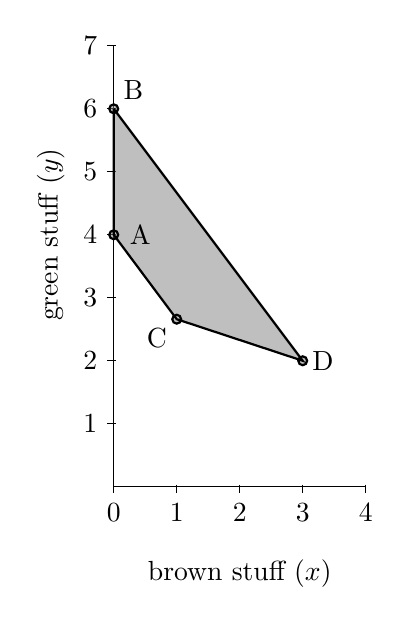
\begin{tikzpicture}[scale=0.8]
  %axis
  \draw (0,0) -- coordinate (x axis mid) (4,0);
  \draw (0,0) -- coordinate (y axis mid) (0,7);
  %ticks
  \foreach \x in {0,...,4}
      \draw (\x,1pt) -- (\x,-3pt);
  \foreach \x in {0,...,4}
      \draw (\x,-3pt) node[anchor=north] {\x};
  \foreach \y in {1,...,7}
      \draw (1pt,\y) -- (-3pt,\y) 
          node[anchor=east] {\y}; 
  %labels      
  \node[below=0.8cm] at (x axis mid) {brown stuff ($x$)};
  \node[rotate=90] at (-1,4) {green stuff ($y$)};
  
  \filldraw[fill=black!50, line width=0.8pt, fill opacity=0.5 ]
    (0,6) -- (0,4) -- (1,2.66) -- (3,2) -- (0,6)
    (0,6) circle (2pt)
    (0,4) circle (2pt)
    (1,2.66) circle (2pt)
    (3,2) circle (2pt);

    \draw (0,6) node[anchor=south west]{B};  
    \draw (.1,4) node[anchor=west]{A};  
    \draw (3,2) node[anchor=west]{D};  
    \draw (1,2.66) node[anchor=north east]{C};  
\end{tikzpicture}
\end{minipage}

}

\vskip 2ex
\noindent 
The solutions of the system $A\bm{x}=\bm{b}$ form a (2-dimensional) plane
in a 5-dimensional space. The variables  $x,y$ represent the amounts
of brown and green stuff, respectively, the variables $s_1,s_2,s_3$
give the slack of the corresponding constraint.
So, for example, the fourth row of the table with constraints $x=s_3=0$
tells us that if the student doesn't buy any brown stuff, and at the same
time he wants to reach the exact allowed intake of aspartame, he has to buy 
6~dl of the green stuff, while he gets more caffeine and sugar than needs.
The last row shows that the constraints can not be added arbitrarily,
but care must be taken not to introduce any linearly dependent rows (in our case
the red and purple lines from the first figure are parallel, so there is no
point in their intersection). In the language of linear programs the rows of
this table are called {\em basic solutions} and those among them that are also
feasible (the highlighted rows) are {\em feasible basic solutions}, and correspond
to the vertices of \dom; in our case the feasible solutions of the program (\ref{eq:LP:2})
form a (2-dimensional) quadrilateral in a 5-dimensional space.

\noindent
It is worth noting that the feasible basic solutions of the program
(\ref{eq:LP:2}), \ie the vertices of the quadrilateral of feasible solutions
in the 5-dimensional space correspond in a straightforward way to the 
vertices of the quadrilateral of the feasible solutions of the program
(\ref{eq:LP:1}): each vertex of the quadrilateral on the right is 
an intersection of two lines corresponding to a constraint  $x_i=0$ 
(and the respective basic solution is feasible). On the other hand, 
every feasible basic solution is the intersection of two such lines.

\vskip 1ex
\noindent
Noting that the introduction of a constraint $x=0$ actually deletes a column
corresponding to the variable $x$ from the respective equation system, 
we arrive to the following definition:

\begin{ozn}
Let  $A\in\R^{m\times n}$ be a matrix with  $m$ rows and $n$ columns. Given a set
$B\subseteq\{1,2,\ldots,n\}$, the symbol $A_B$ denotes the submatrix of $A$
consisting of columns indexed by the set $B$. The same notation
$\bm{x}_B$ 
will be used for vectors.
\end{ozn}

\noindent
For example,
\begin{align*}
A&=\left(\begin{array}{ccccc}-30&-90&1&0&0\\-40&-30&0&1&0\\30&40&0&0&1\end{array}\right)
 &A_{\{1,2\}}&=\left(\begin{array}{ccccc}-30&-90\\-40&-30\\30&40\end{array}\right)
 &A_{\{3,4,5\}}&=\left(\begin{array}{ccccc}1&0&0\\0&1&0\\0&0&1\end{array}\right)
\end{align*}


\begin{framed} 
  \begin{dfn} 
    \label{dfn:LP:basis} 
    Consider a linear program in the normal form, where
    $A\in\R^{m\times n}$.
    A {\bfseries basic solution} is a vector  $\bm{x}\in\R^n$, 
    for which there is an $m$-element set
    $B\subseteq\{1,\ldots,n\}$ such that
    \begin{enumerate}
      \item the matrix $A_B\in\R^{m\times m}$ has full rank, $m$ (\ie is non-singular)
      \item $x_j=0$ for all $j\not\in B$
    \end{enumerate}
  \end{dfn}
\end{framed}

\noindent 
Now let us show that our definition of a basic solution is good in the sense that
in order to find the optimal solution it is sufficient to check the feasible basic
solutions:


\begin{veta}
Consider a linear program in the normal form, such that the 
value of the utility function  $\bm{c}\tr\bm{x}$ is bounded from
above on the polyhedron \dom. Then for every feasible solution $\bm{x_0}$
there is some feasible basic solution $\bm{\tilde{x}}$,
for which
$\bm{c}\tr\bm{\tilde{x}}\ge\bm{c}\tr\bm{x_0}$.
\end{veta}

\begin{dokaz}
  Let us take any feasible solution $\bm{x_0}$, and consider all 
  feasible solutions  $\bm{x}$, for which $\bm{c}\tr\bm{x}\ge\bm{c}\tr\bm{x_0}$.
  Let $\bm{\tilde{x}}$ the one from them with the largest number of zero coordinates.
  We show that $\bm{\tilde{x}}$ is basic. If  $\bm{\tilde{x}}=\bm{0}$,
  it is clearly basic. So let us suppose that  $\bm{\tilde{x}}$ has at least
  one non-zero coordinate. Let us denote by
  $K=\left\{j\in\{1,\ldots,n\}\mid\tilde{x}_j>0\right\}$
  the set of all positive (a feasible solution has no negative coordinates) coordinates
   of the vector $\bm{\tilde{x}}$. Subsequently, let us distinguish two cases:

\bulpar {\em The columns of the matrix $A_K$ are linearly independent.} Clearly $|K|\le m$
(the matrix $A$ has $m$ rows). If $|K|=m$, 
according to the Definition~\ref{dfn:LP:basis}, $\bm{\tilde{x}}$ has $\tilde{x_j}=0$
for all $j\not\in K$, and the matrix $A_K$ is non-singular. 
If $|K|<m$, 
the $|K|$ columns of $A_K$ can be augmented with $m-k$ columns from $A$ in such a way to be
linearly independent\footnote{This claim is covered in the introductory algebra course.}.
Hence, we arrive at a set $K'$, so that $|K'|=m$, $A_{K'}$ is non-singular, and  $\tilde{x_j}=0$ 
for all
$j\not\in K'\supseteq K$.

\bulpar {\em The columns of the matrix $A_K$ are linearly dependent,} 
which means that there is a vector
$\bm{\vartheta}\in\R^{|K|}$ such that $A_K\bm{\vartheta}=\bm{0}$
(\bm{\vartheta} 
determines the linear combination of the columns of $A_K$ that yields the
zero vector).
Let us extend \bm{\vartheta} to $n$-dimensional vector \bm{w} 
by letting all coordinates not in $K$ be zero, so that 
$\bm{w}_K=\bm{\vartheta}$, and
$A\bm{w}=0$.  For any real $t\ge0$, let us denote
$\bm{x}(t)=\bm{\tilde{x}}+t\bm{w}$.  Since $\bm{\tilde{x}}$ 
is a feasible solution, it holds
$A\bm{\tilde{x}}=\bm{b}$. At the same time we have $A\bm{w}=\bm{0}$, and so
also $A\bm{x}(t)=\bm{b}$.

Before concluding the proof, let us modify the vector \bm{w} so that
$\bm{c}\tr\bm{w}\ge0$, and at the same time $w_j<0$ for some $j\in K$:
If $\bm{c}\tr\bm{w}=0$, and for all $j\in K$ it holds  $w_j>0$, 
it is sufficient to multiply 
\bm{w}
by -1, and we have the required form. So let it hold
$\bm{c}\tr\bm{w}\not=0$.
If  $\bm{c}\tr\bm{w}<0$, the \bm{w} 
can be again multiplied by -1, so without loss of generality we can suppose
that 
$\bm{c}\tr\bm{w}>0$. 
Let us show that now there must exist some
$j\in K$, for which $w_j<0$.
If it is not the case, \ie if for all $j\in K$ it holds $w_j>0$,
clearly it must be that  $\bm{w}\ge\bm{0}$  (the coordinates
$i\not\in K$ have been padded by zeroes).
But then
$\bm{x}(t)=\bm{\tilde{x}}+t\bm{w}\ge0$ for all $t\ge0$, so that
$\bm{x}(t)$ is a feasible solution. The utility function has value
$\bm{c}\tr\bm{x}(t)=\bm{c}\tr\bm{\tilde{x}}+t\bm{c}\tr\bm{w}$. Since
$\bm{c}\tr\bm{w}>0$, for $t\mapsto\infty$ is $\bm{c}\tr\bm{x}(t)\mapsto\infty$,
and hence the original linear program was not bounded.

\noindent
Now let us have the vector \bm{w} in the form where $\bm{c}\tr\bm{w}\ge0$,
and at the same time $w_j<0$ for some $j\in K$.
We show that for some  $t_1>0$, the vector $\bm{x}(t_1)$
is a feasible solution with more zero coordinates than $\bm{\tilde{x}}$.
However, this contradicts the fact that  $\bm{\tilde{x}}$ has the most
zero coordinates from among all feasible solutions $\bm{x}$ for which
$\bm{c}\tr\bm{x}\ge\bm{c}\tr\bm{x_0}$, since 
$\bm{c}\tr\bm{x}(t_1)=\bm{c}\tr\bm{\tilde{x}}+t_1\bm{c}\tr\bm{w}\ge\bm{c}\tr\bm{x_0}$
(because $\bm{c}\tr\bm{\tilde{x}}\ge\bm{c}\tr\bm{x_0}$ a $\bm{c}\tr\bm{w}\ge0$).

The vector $\bm{x}(t_0)=\bm{\tilde{x}}$ 
is feasible, and has coordinates $j\in K$ (strictly) positive,
ant the remaining ones zero. At the same time we know that there is at least one
$j\in K$ for which  $w_j<0$.
Since the $j$-th coordinate of  $\bm{x}(t)$ is $x(t)_j=\tilde{x}_j+tw_j$,
with increasing $t$ the values  $x(t)_j$
are decreasing for all $j$ for which $w_j<0$. Denote $t_1$ the value $t$ when the first
of the values  $x(t)_j$ reaches zero. Clearly,  $\bm{x}(t_1)$
is feasible, and has more zero coordinates than  $\bm{\tilde{x}}$.
\end{dokaz}

\noindent 
The consequence of this theorem is that in order to find the optimal solution
of a linear program with finite optimum, it is sufficient to check all 
feasible basic solutions. This is a generalization of the approach from the
introductory example with two dimensions, where it was sufficient to check
the vertices of a suitable polygon. How to find the basic solutions?
Just note that for a given set 
$B\subseteq\{1,\ldots,n\}$ 
there is at most one basic solution
\footnote{The other direction does not hold, the same basic solution \bm{x}
  can be possibly obtained from different sets $B$, $B'$. If, e.g., the 
  vector \bm{0} is feasible, it is also a feasible solution for any basis
$B$.}: if there were two basic solutions  $\bm{y},\bm{z}$ with the same set $B$,
it must hold $A\bm{y}=A\bm{z}=\bm{b}$ and so $A_B\bm{y}=A_B\bm{z}=\bm{b}$.
Since $A$ is a non-singular square matrix, the equation system $A_B\bm{x}=\bm{b}$ 
has a unique solution, and hence $\bm{y}=\bm{z}$.
It means that it is sufficient to try all sets $B$< check it the corresponding $A_B$ is non-singular
(e.g., by Gaussian elimination), check if the solution  $A_B\bm{x}=\bm{b}$ is feasible, and choose
the best of such feasible \bm{x}.
The problem, of course, is that with $n$ variables, and $m$ constraints, one has potentially ${n\choose m}$
distinct basis solutions, so the algorithm that checks all of them is not polynomial
\footnote{For, say, $m=n/2$, we get from Stirling approximation 
  $n!\approx\sqrt{2\pi n}\left(\frac{n}{e}\right)^n\left(1+o(n)\right)$ 
 that 
\hbox{$\left(n\atop \frac{n}{2}\right)=\frac{n!}{\left[\left(\frac{n}{2}\right)!\right]^2}\ge 2^n/n^2$.}}.
In the next chapter we show how to solve the linear programming problem in a more efficient way using
the simplex method.


